\chapter{Results and Discussion}
\label{chp:Results and Discussion}
This chapter documents the results from the trial conducted on the Ear-Monitor. The aim is to quantify the level of comparability between the Ear-Monitor's and benchmark device's measurements and through this get an understanding of the level of accuracy of the Ear-Monitor's measurements. Each participant is acting as his/her own control is this type of analysis. Results are discussed one medical sign at a time in this chapter.

\section{Temperature Results}
During each recording session, 15 Ear-Monitor data points and 3 ET 100-A benchmark data points are collected. It is assumed that the participant's core temperature stays constant during the duration of the recording session. Therefore the average ET 100-A benchmark measurement and the average Ear-Monitor measurement are compared. Two participants' data is removed due to faulty recording sessions.

\medskip

The Ear-Monitor data points are analysed in terms of correlation with the ET 100-A benchmark measurements and the average error. An error is the difference between the ET 100-A benchmark measurement and the Ear-Monitor measurement. Results from the two calibration approaches are documented separately and then compared in the discussion.

\subsection{Calibration Group Results}
Equation \ref{eq:TempCal} is used to calculate tympanic temperature for all participants. Figure \ref{fig:Temp1Scatter} shows a scatter plot of the average Ear-Monitor vs. ET 100-A data points for the 28 recording sessions with temperature measurements. The black line is the $x=y$ line and the blue line is fitted to the data through the least squares method.

\begin{figure}[H]
   \centering
   \includegraphics[width=12cm,height=7.5cm]{figs/Temp1Scatter.png}
   \caption{Temperature through Calibration Group: ET 100-A vs. Ear-Monitor}
   \label{fig:Temp1Scatter}
\end{figure}

The the average error is found to be 0.0160 $\pm$\SI{0.0226}{\celsius} and the average of the absolute value of all the errors is 0.3399 $\pm$\SI{0.0157}{\celsius}.

\subsection{Intra-participant Calibration Results}
This method used the data from the first recording session to calibrate the Ear-Monitor, and the data from the second session is used to evaluate this method. Figure \ref{fig:Temp2Scatter} shows a scatterplot of the average Ear-Monitor vs. ET 100-A data points for the 14 second recording sessions. Again the black line $x=y$ and the blue line is fitted to the data.

\begin{figure}[H]
   \centering
   \includegraphics[width=12cm,height=7.5cm]{figs/Temp2Scatter.png}
   \caption{Temperature through Intra-participant Calibration: ET 100-A vs. Ear-Monitor}
   \label{fig:Temp2Scatter}
\end{figure}

The results of the intra-participant calibration shows an average error of 0.0114 $\pm$\SI{0.0190}{\celsius} and an average of the absolute value of all the errors of 0.2499 $\pm$\SI{0.0087}{\celsius}.

\medskip

The results for the two different calibration methods are summarised in Table \ref{tab:ResultsTemp}. The calibration group method is labelled and A and the intra-participant calibration method as B. The temperature values are recording session averages with standard errors indicated in brackets. All values are in \SI{}{\celsius}.

\begin{table}[H]
\caption{Summary of the temperature results}
\label{tab:ResultsTemp}
\centering
\begin{tabular}{|P{1.4cm} | P{1.4cm} || P{1.6cm} |P{1.2cm}| |P{1.6cm} |P{1.2cm}|P{2cm}|} 
\hline
Partici-pant No.	&	ET 100-A Temp	&	Ear-Monitor Temp A	&	Error A	&	Ear-Monitor Temp B	&	Error B	&	Ear-Monitor standard error\\
\hline
2a	&	36.33	&	37.63 	&	-1.29	&	-		&	-		&	$\pm$0.0043\\
2b	&	36.37	&	37.57 	&	-1.21	&	36.08	&	0.28	&	$\pm$0.0017\\
3a	&	37.65	&	37.54 	&	0.11	&	-		&	-		&	$\pm$0.0031\\
3b	&	37.40	&	37.67 	&	-0.27	&	37.58	&	-0.18	&	$\pm$0.0172\\
4a	&	38.30	&	37.37 	&	0.93	&	-		&	-		&	$\pm$0.0012\\
4b	&	38.55	&	37.44 	&	1.11	&	38.17	&	0.38	&	$\pm$0.0014\\
6a	&	38.35	&	37.80 	&	0.55	&	-		&	-		&	$\pm$0.0032\\
6b	&	37.60	&	37.76 	&	-0.16	&	38.11	&	-0.51	&	$\pm$0.0015\\
7a	&	37.03	&	37.31 	&	-0.28	&	-		&	-		&	$\pm$0.0008\\
7b	&	37.00	&	37.34 	&	-0.34	&	36.86	&	0.14	&	$\pm$0.0016\\
8a	&	38.40	&	38.13 	&	0.27	&	-		&	-		&	$\pm$0.0072\\
8b	&	38.50	&	38.03 	&	0.47	&	38.10	&	0.40	&	$\pm$0.0009\\
9a	&	37.55	&	37.53 	&	0.02	&	-		&	-		&	$\pm$0.0005\\
9b	&	37.40	&	37.54 	&	-0.14	&	37.36	&	0.04	&	$\pm$0.0007\\
10a	&	37.95	&	37.70 	&	0.25	&	-		&	-		&	$\pm$0.0031\\
10b	&	38.10	&	37.73 	&	0.37	&	37.77	&	0.33	&	$\pm$0.0007\\
11a	&	37.50	&	37.52 	&	-0.02	&	-		&	-		&	$\pm$0.0006\\
11b	&	37.60	&	37.50 	&	0.10	&	37.27	&	0.33	&	$\pm$0.0051\\
12a	&	38.50	&	38.51 	&	-0.01	&	-		&	-		&	$\pm$0.021\\
12b	&	37.70	&	38.18 	&	-0.48	&	37.97	&	-0.27	&	$\pm$0.0028\\
13a	&	38.05	&	38.02 	&	0.03	&	-		&	-		&	$\pm$0.012\\
13b	&	37.53	&	37.92 	&	-0.39	&	37.75	&	-0.22	&	$\pm$0.0016\\
14a	&	38.00	&	37.73 	&	0.27	&	-		&	-		&	$\pm$0.001\\
14b	&	37.95	&	37.75 	&	0.20	&	37.82	&	0.13	&	$\pm$0.0004\\
15a	&	37.65	&	37.58 	&	0.07	&	-		&	-		&	$\pm$0.0033\\
15b	&	37.30	&	37.55 	&	-0.25	&	37.42	&	-0.12	&	$\pm$0.0008\\
16a	&	37.90	&	37.90 	&	0.00	&	-		&	-		&	$\pm$0.0016\\
16b	&	37.50	&	37.93 	&	-0.43	&	37.73	&	-0.23	&	$\pm$0.0038\\
\hline
\end{tabular}
\end{table}

\subsection{Temperature Results Discussion}
It is clear form the Ear-Monitor standard errors in Table \ref{tab:ResultsTemp} that the TMP006 has a high precision. The measurements inside a recording session are close to one another, with the maximum standard error being $\pm$ \SI{0.0172}{\celsius}. This was expected owing to the thermal consistency inside the ear canal. Air flow is negligible and the position of objects in the sensor's field of vision stays constant. These factors contrite to high precision measurements.

\medskip

The two different calibration methods can be compared through a box and whisker plot of their respective errors as can be seen in Figure \ref{fig:ComparingCalibrationBoxplot}. 

\begin{figure}[H]
   \centering
   \includegraphics[width=12cm,height=7.5cm]{figs/ComparingCalibrationBoxplot.png}
   \caption{Temperature errors of Calibration group method and Intra-participant calibration method}
   \label{fig:ComparingCalibrationBoxplot}
\end{figure}

The methods used to analyse the data unanimously indicate that the intra-participant calibration method is superior to the group calibration method with regards to accuracy. The scatter plots, Figure \ref{fig:Temp1Scatter} and \ref{fig:Temp2Scatter}...

Compare errors
Mention standard errors are unchanged
Add ICC values
Evaluate ear-monitors ability to measure temp
Compare to other word/devices (Cosinuss)


%---------------------------------------------------------------------------------------------------------------------------------------------

\section{Heart Rate Results}
The Ear-Monitor uses an IR PPG obtained for the ear canal to detect pulse peaks via a beat detection algorithm. The average period between 10 successive detected beats are used to calculate the heart rate. The beat detection algorithm is at the core of the heart rate functionality of the Ear-Monitor, and therefore it is be evaluated independently. This is followed by comparative analysis between the individual beat periods and 10-beat moving average heart rates of the Ear-Monitor and Nexus-10 physiological monitor.

\subsection{Beat Detection Algorithm Evaluation Results}
The beat detection algorithm used by the Ear-Monitor is first tested on open source data from PhysioNet.org, and then on the data collected during the trial. These results of these two tests are discussed separately. 

\subsubsection{PhysioNet Data Test}
The beat detection algorithm is PPG data from the open-source MIMIC Database on PhysioNet.org \citep{PhysioNet}. This data was recorded from patients in intensive care units and is made available for developing and testing intelligent monitoring systems. PPG data is recorded with clinical finger pulse oximeters.

\medskip

Ten minute segments of 14 different patients are used to test the algorithm. Each set of data also includes an ECG signal, which is used to identify the benchmark beats. Table \ref{tab:PhysioNet} summarises the results from this test.

\begin{table}[H]
\caption{Results of the beat detection algorithm on the PhysioNet data}
\label{tab:PhysioNet}
\centering
\begin{tabular}{|P{3cm}| P{3cm}| P{3cm} |P{3cm}|} 
\hline
Record No.	&	Actual No. Beats	&	False Positives	&	False negatives\\ 
\hline
039		&	1337				&	0				&	0\\
\hline
041		& 	1030				&	1				&	7\\
\hline
055		&	1021				&	0				&	0\\
\hline
211		&	891					&	2				&	8\\
\hline
212		&	845					&	0				&	15\\
\hline
216		&	763					&	0				&	1\\
\hline
218		&	697					&	0				&	1\\
\hline
219		&	720					&	0				&	0\\
\hline
221		&	776					&	0				&	4\\
\hline
224		&	863					&	0				&	0\\
\hline
230		&	871					&	7				&	36\\
\hline
237		&	777					&	2				&	17\\
\hline
240		&	816					&	1				&	2\\
\hline	
252		&	594					&	0				&	0\\
\hline
\end{tabular}
\end{table}

Of the 12001 beats in all the test data, 13 (0.108\%) false positives were detected and 91 (0.758\%) false negatives. Even though the beat-detection algorithm was designed and tuned using PPGs collected form the ear canal wall, it can accurately detect beats from finger pulse oximeters. This results demonstrates the robustness of the algorithm. Most false detections occurred where signals were corrupted by noise. It also illustrate how the SSF can extract beats, even from a noisy signal by including a plot of the PPG and subsequent SSF plus detected beats.

\subsubsection{Trial Data Test}
Next the algorithm is tested using the data collected during the trial. The number of beats detected by the Ear-Monitor will be compared to the actual number of heartbeats. The Nexus-10's supporting software, BioTrace+, has a peak detection algorithm, but it was found that is misses some peaks. To ensure accurate benchmark peak detection, the PPG from the Nexus-10 is inspected manually and peaks are marked by a human annotator. Figure \ref{BeatDetectionTest} shows plots of (a) the Ear-Monitor SSF with detected beats and (b) the Nexus-10 PPG signal with annotated beats. In this example 100\% of the peaks are detected by Ear-Monitor.

\begin{figure}[H]
   \centering
   \includegraphics[width=12cm,height=7.5cm]{figs/BeatDetectionTest.png}
   \caption{Plots of (a) the Ear-Monitor SSF with detected beats and (b) the Nexus-10 PPG signal with annotated beats} %Marga1_Data
   \label{fig:BeatDetectionTest}
\end{figure}

Table \ref{tab:BeatDetectionTest} summarises the results to the beat detection evaluation.

\begin{table}[H]
\caption{Results of the beat detection algorithm on the PhysioNet data}
\label{tab:BeatDetectionTest}
\centering
\begin{tabular}{|P{1.9cm}| P{1.9cm}| P{1.9cm} | P{1.9cm} | P{1.9cm} | P{1.9cm} |} 
\hline
Participant No.	&	 No. Nexus-10 Beats	&	No. Ear-Monitor Beats	&	False Positives & False Negatives & \%\\ 
\hline
1a	&	150	&	150	&	0	&	0	&	100	\\
\hline
1b	&	148	&	148	&	0	&	0	&	100	\\
\hline
2a	&	116	&	108	&	2	&	10	&	93.1	\\
\hline
2b	&	116	&	106	&	1	&	11	&	91.4	\\
\hline
3a	&	136	&	136	&	0	&	0	&	100	\\
\hline
3b	&	138	&	138	&	0	&	0	&	100	\\
\hline
4a	&	132	&	132	&	0	&	0	&	100	\\
\hline
4b	&	133	&	132	&	0	&	1	&	99.2	\\
\hline
5a	&	181	&	181	&	0	&	0	&	100	\\
\hline
5b	&	188	&	187	&	0	&	1	&	99.5	\\
\hline
6a	&	120	&	120	&	0	&	0	&	100	\\
\hline
6b	&	127	&	127	&	0	&	0	&	100	\\
\hline
7b	&	144	&	144	&	0	&	0	&	100	\\
\hline
7c	&	140	&	140	&	0	&	0	&	100	\\
\hline
8a	&	163	&	163	&	0	&	0	&	100	\\
\hline
8b	&	164	&	163	&	0	&	1	&	99.4	\\
\hline
9a	&	149	&	149	&	0	&	0	&	100	\\
\hline
9b	&	146	&	142	&	0	&	4	&	97.3	\\
\hline
10a	&	146	&	146	&	0	&	0	&	100	\\
\hline
10c	&	146	&	146	&	0	&	0	&	100	\\
\hline
11a	&	131	&	131	&	0	&	0	&	100	\\
\hline
11b	&	131	&	131	&	0	&	0	&	100	\\
\hline
12a	&	144	&	144	&	0	&	0	&	100	\\
\hline
12b	&	137	&	137	&	0	&	0	&	100	\\
\hline
13a	&	169	&	163	&	0	&	6	&	96.45	\\
\hline
13b	&	169	&	162	&	0	&	7	&	95.86	\\
\hline
14a	&	168	&	168	&	0	&	0	&	100	\\
\hline
14b	&	170	&	170	&	0	&	0	&	100	\\
\hline
15a	&	149	&	149	&	0	&	0	&	100	\\
\hline
15c	&	149	&	149	&	0	&	0	&	100	\\
\hline
16a	&	154	&	151	&	1	&	4	&	98.05	\\
\hline
16b	&	159	&	152	&	6	&	13	&	95.6	\\
\hline
\end{tabular}
\end{table}

Of the 4713 beats in all the participant trail data, 4655 (98.77\%) are successfully detected. 10 (0.21\%) false positives and 58 (1.23\%) false negatives are detected. It should also be noted the 51 of the false negatives are from the data collected from three of the participants.

Figure \ref{fig:BeatDetectionScatter} shows a scatted plot of the number of annotated Nexus-10 beats vs. the number of detected Ear-Monitor beats. Data recording sessions from all 16 trial participants are used, meaning 32 sets of data points are compared.

\begin{figure}[H]
   \centering
   \includegraphics[width=12cm,height=7.5cm]{figs/BeatDetectionScatter.png}
   \caption{Number of beats: Nexus-10 vs. Ear-Monitor}
   \label{fig:BeatDetectionScatter}
\end{figure}

This test shows that the Ear-Monitor preforms well in its task of detection beats. The number of false negatives detected for the trial data is higher than for the PhysioNet data. This can be ascribed to the fact that the PPG from three of the participants was of a notably lower quality. Although the adaptive threshold method detected the majority if the peaks, the amplitude of the SSF peaks varied prominently and very low amplitudes were missed by the algorithm. This can be caused by low blood profusion in the ear canal or bad contact between the MAX30100 and the canal wall. This is a patient specific inaccuracy and can be overcome by an more customised ear probe. 

\subsection{Beat Period and Average Heart Rate Results}
The accuracy of the heat beat period is tested to see if beats and detected at the right position in time. The individual period between beats detected be the Ear-Monitor is compared to the period between beats annotated on the Nexus-10 PPG. Figure \ref{fig:PeriodScatter} shows a scatter plot of the Nexus-10 period vs. theEar-Monitor period. A total of 4569 periods are compared from all 16 participants.

\begin{figure}[H]
   \centering
   \includegraphics[width=12cm,height=7.5cm]{figs/PeriodScatter.png}
   \caption{Beat period: Nexus-10 vs. Ear-Monitor}
   \label{fig:PeriodScatter}
\end{figure}

The 10-beat average heart rate is calculate form the Ear-Monitor and Nexus-10 data and compared in the same way as with he beat periodes. Figure \ref{fig:HeartRateScatter} shows a scatter plot of the Nexus-10 heart rate vs. the Ear-Monitor heart rate. A total of 4258 periods are compared from all 16 participants.

\begin{figure}[H]
   \centering
   \includegraphics[width=12cm,height=7.5cm]{figs/HeartRateScatter.png}
   \caption{10-beat average heart rate: Nexus-10 vs. Ear-Monitor}
   \label{fig:HeartRateScatter}
\end{figure}

\subsection{Heart Rate Results Discussion}
Blablabla...


%---------------------------------------------------------------------------------------------------------------------------------------------

\section{Respiratory Rate Results}
The Ear-Monitor uses respirators sinus arrhythmia, the frequency modulating respiratory heart rate characteristic, to extract a respiratory rate. The the chest strap connected to the Nexus-10 physiological monitoring platform is used to measure the benchmark respiration rate. Benchmark breaths from the Nexus-10 are manually annotated. The recording session consisted of one minute of normal breathing followed by one minute of breathing regulated at 15 breaths per minute. Table \ref{tab:RSP_Data} shows a summary of the breaths detected during all recording sessions.%Data from all 16 participants is used to compile the respiratory rate results. 

\begin{table}[H]
\caption{Summery of breaths recorded during each recording session}
\label{tab:RSP_Data}
\centering
\begin{tabular}{|P{1.9cm}|P{3.2cm}|P{3.2cm}|P{1.2cm}|} 
\hline
Participant No.	&	No. Nexus-10 Breaths	&	No. Ear-Monitor Breaths	&	Error	\\
\hline
1a	&	30	&	30	&	0	\\
1b	&	23	&	22	&	1	\\
2a	&	27	&	22	&	5	\\
2b	&	27	&	22	&	5	\\
3a	&	28	&	25	&	3	\\
3b	&	25	&	25	&	0	\\
4a	&	28	&	29	&	-1	\\
4b	&	28	&	27	&	1	\\
5a	&	24	&	33	&	-9	\\
5b	&	24	&	44	&	-20	\\
6a	&	34	&	29	&	5	\\
6b	&	32	&	30	&	2	\\
7b	&	28	&	29	&	-1	\\
7c	&	26	&	26	&	0	\\
8a	&	29	&	27	&	2	\\
8b	&	29	&	32	&	-3	\\
9a	&	42	&	31	&	11	\\
9b	&	43	&	29	&	14	\\
10a	&	31	&	29	&	2	\\
10b	&	32	&	32	&	0	\\
11a	&	29	&	28	&	1	\\
11b	&	29	&	28	&	1	\\
12a	&	32	&	26	&	6	\\
12b	&	34	&	33	&	1	\\
13a	&	30	&	39	&	-9	\\
13b	&	28	&	43	&	-15	\\
14a	&	22	&	22	&	0	\\
14b	&	23	&	24	&	-1	\\
15a	&	32	&	32	&	0	\\
15c	&	30	&	33	&	-3	\\
16a	&	29	&	28	&	1	\\
16b	&	35	&	33	&	2	\\
\hline
\end{tabular}
\end{table}

\medskip
It should be noted, however, that the majority of the inaccuracy can be traced to the recording sessions participants 5, 9 and 13. Upon closer inspection the following explanation can be given. Participant 5 and 13 both has a large number of false positives, the highest and third highest average heart rates and very low heart beat period variation due to RSA. Participant 9 has an unusually high resting respiratory rate (more than double that of the average of the rest of the participants), bordering on the maximum measurable rate according to the Nyquist theorem, which is equal to half the heart rate. This caused 51\% of breaths to be missed during normal breathing. As expected, when the respiratory rate was raised during the controlled breathing exercise, the breath detection accuracy returned to the group average. These three participants are regarded as outliers and are isolated from the rest in order to reveal the trends present the bulk of the recording sessions.

\medskip

The average errors in respiratory rate between the benchmark Nexus-10 and the Ear-Monitor can be seen in Table \ref{tab:BreathingAccuracies}. Standard deviations are included and all values are in breaths per minute. By removing the outliers the average error of the normal and controlled breathing groups are closer to one another and the standard deviation in the errors are reduced by more than half.

\begin{table}[H]
\caption{Average errors of the respiratory rate measurements}
\label{tab:BreathingAccuracies}
\renewcommand{\arraystretch}{1.2}
\centering
\begin{tabular}{|P{4cm}|P{4cm}|P{4cm}|} 				
\hline
Group				&	Outliers removed		&	Outliers included\\ 
\hline
Normal breathing	&	-0.6154 $\pm$0.3285		&	0.4375 $\pm$0.8694\\
%\hline
Breathing exercise 	&	-0.5000 $\pm$0.2166		&	-0.40625$\pm$0.4327\\
%\hline
All					&	-0.5577 $\pm$0.1950		&	0.0156 $\pm$0.4846\\
\hline
\end{tabular}
\end{table}

Figure \ref{fig:BreathScatter} shows a plot of the Nexus-10's benchmark breaths versus the Ear-Monitor's detected breaths. Blue marks the number of breaths after 1 minute of normal breathing and red marks the total number of breaths in the recording session, including the  breathing exercise.

\begin{figure}[H]
   \centering
   \includegraphics[width=12cm,height=7.5cm]{figs/BreathScatter.png}
   \caption{Number of breaths detected: Nexus-10 vs. Ear-Monitor}
   \label{fig:BreathScatter}
\end{figure}

\subsection{Respiratory Rate Discussion}
The breathing exercise was included in the trail, due to the uncertainty that the RSA will be visible during normal breathing. In general, participants started breathing deeper during the breathing exercise. This resulted in a more accurate detection of breaths.

\medskip

Although the standard deviation for the data from the breathing exercise is lower, the Ear-Monitor sill measured respiratory rate during normal breathing better than expected. According to the trial data (excluding th outliers), the Ear-Monitor is able to calculate the respiratory rate of a participant breathing normally to with in an average accuracy of -0.6154 breaths per minute with a standard precision of $\pm$ 0.3285 breaths per minute (6.78\% standard deviation at 14 breaths per minute). This is superior to the 1 breath per minute accuracy from \cite{clifton2007measurement} and the 7.6\% accuracy from \cite{leonard2006fully}.

\medskip

It can be seen that, on average, the Ear-Monitor detects a respiratory rate that is slightly lower (-0.5577 $\pm$0.1950 breaths per minute) than the actual rate. This means that the algorithm misses some breaths. This can be ascribed to intermitted shallower and shorter breaths that does not cause an big enough variation in heart beat period.

\medskip

The outliers are removed to emphasize the normal results, but they are not random and provide a valuable insight into the limitations of using RSA to measure respiratory rate. Is can be stated that elevated heart rates (higher than 80 bpm in this trial) reduces the magnitude of RSA  and causes the detection of false breaths. Also, if the breathing rate approaches half the heart rate (Nyquist theorem), the sample frequency is to low and many breaths are missed by the detection algorithm. These results can be summarised by saying that respiratory rate measurement through RSA is most accurate at lower heart and respiratory rates.

